% !TeX spellcheck = en_GB
\documentclass[10pt,usenames,dvipsnames]{beamer}
\usetheme{CambridgeUS}
%\usetheme{Boadilla}
\definecolor{myred}{RGB}{163,0,0}
%\usecolortheme[named=`blue]{structure}
\usecolortheme{dove}
\usefonttheme[]{professionalfonts}
\usepackage[english]{babel}
\usepackage{amsmath,amsfonts,amssymb}
\usepackage{xcolor}
\usepackage{tikz}
\usepackage{pgfplots}
\pgfplotsset{compat=newest,compat/show suggested version=false}
\usetikzlibrary{matrix,overlay-beamer-styles,arrows,shapes,calc,backgrounds}
\usepackage{bm}
\usepackage{textcomp}
\usepackage{gensymb}
\usepackage{verbatim}
\usepackage{paratype}
\usepackage{mathpazo}
\usepackage{listings}
\usepackage{csvsimple}

\newcommand{\cov}{\mathsf{cov}}
\newcommand{\corr}{\mathsf{corr}}
\newcommand{\var}{\mathsf{Var}}
\newcommand{\plim}{\mathrm{plim\ }}
\newcommand{\E}{\mathsf{E}}
\newcommand{\Est}{\mathsf{Est.Var}}
\newcommand{\Asy}{\mathsf{Asy.Var}}
\newcommand{\Esta}{\mathsf{Est.Asy.Var}}
\newcommand{\tr}{\mathrm{tr}}
\newcommand{\Prob}{\mathrm{Prob}}
\newcommand{\Med}{\mathsf{Med}}
\newcommand{\rank}{\mathsf{rank}}
\newcommand{\argmin}{\mathsf{arg\,min}}

\newcommand{\cc}[1]{\texttt{\textcolor{blue}{#1}}}

\definecolor{ttcolor}{RGB}{0,0,1}%{RGB}{163,0,0}

% Number theorem environments
\setbeamertemplate{theorem}[ams style]
\setbeamertemplate{theorems}[numbered]

% Reset theorem-like environments so that each is numbered separately
%\usepackage{etoolbox}
%\undef{\definition}
\theoremstyle{plain}
\newtheorem{thm}{Theorem}
\newtheorem{Fact}{\translate{Fact}}
\theoremstyle{definition}
\newtheorem{defn}{\translate{Definition}}
\newtheorem{exmpl}{\translate{Example}}

\definecolor{ttcolor}{RGB}{0,0,1}%{RGB}{163,0,0}
\definecolor{mygray}{RGB}{248,249,250}

% Change colours for theorem-like environments
\definecolor{mygreen1}{RGB}{0,96,0}
\definecolor{mygreen2}{RGB}{229,239,229}
\setbeamercolor{block title}{fg=white,bg=mygreen1}
\setbeamercolor{block body}{fg=black,bg=mygreen2}

\lstdefinestyle{numbers}{numbers=left, stepnumber=1, numberstyle=\tiny, numbersep=10pt}
\lstdefinestyle{MyFrame}{backgroundcolor=\color{yellow},frame=shadowbox}

\lstdefinestyle{rstyle}%
{language=R,
	basicstyle=\footnotesize\ttfamily,
	backgroundcolor = \color{mygray},
	commentstyle=\slshape\color{green!50!black},
	keywordstyle=\bfseries\color{blue!50!black},
	identifierstyle=\color{blue},
	stringstyle=\color{orange},
	%escapechar=\#,
	rulecolor = \color{mygray}, 
	showstringspaces = false,
	showtabs = false,
	tabsize = 2,
	emphstyle=\color{red},
	frame = single} 

\setbeamertemplate{navigation symbols}{}

\lstset{language=R,frame=single}

\AtBeginSection{\frame{\sectionpage}}

% Remove Section 1, Section 2, etc. as titles in section pages
\defbeamertemplate{section page}{mine}[1][]{%
	\begin{centering}
		{\usebeamerfont{section name}\usebeamercolor[fg]{section name}#1}
		\vskip1em\par
		\begin{beamercolorbox}[sep=12pt,center]{part title}
			\usebeamerfont{section title}\insertsection\par
		\end{beamercolorbox}
	\end{centering}
} 

\setbeamertemplate{section page}[mine]  

\hypersetup{colorlinks, urlcolor=blue, linkcolor = myred} 

\title{R406: Applied Economic Modelling with Python}
\subtitle{\textcolor{myred}{Unconstrained Optimization. Static Optimization with Equality Constraints. Lagrange Multipliers}}
\author[Andrey Vassilev]{Andrey Vassilev}

\date{} 

\begin{document}
\maketitle

\begin{frame}[fragile]
\frametitle{Lecture Contents}
\tableofcontents
\end{frame}


\begin{section}{Warm-up: Basic Unconstrained Optimization in $ \mathbb{R}^1 $}\label{sec:R1}
	
	\begin{frame}[fragile]
		\frametitle{Warm-up: Basic Unconstrained Optimization in $ \mathbb{R}^1 $}
		
		\begin{Fact}
			For a function $ f: \mathbb{R} \rightarrow \mathbb{R} $ differentiable at a point $ x $, a necessary condition for a local extreme point (i.e. a maximum or a minimum) at $ x $ is \[ f'(x) = 0. \]
		\end{Fact}
		\bigskip
		
		\begin{exmpl} %{Example}
			If $ f(x) = ax^2 + bx + c $, then $ f'(x) = 2ax + b $ and the condition $ f'(x)=0 $ yields the familiar $ x=-\frac{b}{2a} $ (recall your high-school days). Depending on the sign of $ a $, this is a maximum or a minimum (What is the relationship?).
		\end{exmpl}\bigskip
		
		\begin{exmpl} %{Example}
			If $ f(x) = x^3 $, then $ f'(x)=3x^2 $ and $ f'(x)=0 \Rightarrow x=0$.
			
			Does the function attain a maximum or a minimum at $ x=0 $?
		\end{exmpl}
	\end{frame}
	
	\begin{frame}[fragile]
		\frametitle{Warm-up: Basic Unconstrained Optimization in $ \mathbb{R}^1 $}
		\begin{figure}
			\centering
			\includegraphics[width=0.9\linewidth]{cubicfun}
			\label{fig:cubicfun}
		\end{figure}
	\end{frame}
	
	\begin{frame}[fragile]
		\frametitle{Warm-up: Basic Unconstrained Optimization in $ \mathbb{R}^1 $}
		\addtocounter{theorem}{-1}
		\begin{exmpl}[cont.]
			The answer is ``neither''! The point $ x=0 $ is not a local extreme point of $ f(x)=x^3 $.\medskip
			
			This illustrates the pitfalls of using necessary conditions -- they supply only candidates that need to be checked further.
		\end{exmpl}
		
		The above examples generalize in the following manner:
		\begin{Fact}
			Let a function $ f $ be $ n $ times differentiable at a point $ x $ and 
			\[ f'(x)=f''(x)=\ldots=f^{(n-1)}(x)=0,\qquad f^{(n)}\neq 0. \] \vskip -5pt
			\begin{enumerate}
				\item If $ n $ is odd, the point $ x $ is not an extreme point of $ f(x) $.
				\item If $ n $ is even and $ f^{(n)}(x)>0 $, the point $ x $ is a minimum.
				\item If $ n $ is even and $ f^{(n)}(x)<0 $, the point $ x $ is a maximum.
			\end{enumerate}
			\label{fc:SCsR1}
		\end{Fact}
	\end{frame}
	
\end{section}

\begin{section}{Unconstrained Optimization in $ \mathbb{R}^n $}\label{sec:Rn}
	
	\begin{frame}[fragile]
		\frametitle{Unconstrained Optimization in $ \mathbb{R}^n $}
		\framesubtitle{Necessary conditions}
		\begin{Fact}
			For a function $ f: \mathbb{R}^n \rightarrow \mathbb{R}$, differentiable at a point $ \mathbf{x} $, a necessary condition for $ \mathbf{x} $ to be a local extreme point is \[ f'(\mathbf{x}) = \mathbf{0}, \]
			where \[ \mathbf{x} = \left( \begin{array}{c}
				x_1 \\
				x_2\\
				\vdots \\
				x_n
			\end{array}\right),~\mathbf{0} = \left( \begin{array}{c}
				0 \\
				0 \\
				\vdots \\
				0
			\end{array}\right)\text{ and }  f'(\mathbf{x})  = \left( \begin{array}{c}
				\dfrac{\partial f(x_1,\ldots,x_n)}{\partial x_1}\\
				\vdots \\
				\dfrac{\partial f(x_1,\ldots,x_n)}{\partial x_n}
			\end{array}\right)(= \nabla f(\mathbf{x})) \]
			\label{fc:NCsRn}
		\end{Fact}
		
		\textbf{Note:} A point where the gradient of a function $ f $ vanishes is called a \emph{critical point} or a \emph{stationary point}. This also applies to functions on $ \mathbb{R}^1 $.
	\end{frame}
	
	\begin{frame}[fragile]
		\frametitle{Unconstrained Optimization in $ \mathbb{R}^n $}
		\begin{exmpl}
			\[ f(x,y) = x^2 +2y^2-3x+xy \]
			\[ \frac{\partial f}{\partial x} = 2x-3+y=0\quad \Rightarrow \quad x=\frac{3-y}{2} \]
			\[ \frac{\partial f}{\partial y} = 4y+x = 0\quad \Rightarrow \quad y = -\frac{x}{4}\]
			\[ x=\frac{12}{7},~y=-\frac{3}{7} \]
			\label{ex:locminR2}
		\end{exmpl}
	\end{frame}
	
	\begin{frame}[fragile]
		\frametitle{Unconstrained Optimization in $ \mathbb{R}^n $}
		\begin{figure}
			\centering
			\includegraphics[width=0.9\linewidth]{quadformplot}
			\label{fig:quadformplot}
		\end{figure}
	\end{frame}
	
	\begin{frame}[fragile]
		\frametitle{Unconstrained Optimization in $ \mathbb{R}^n $}
		The necessity of the condition $  f'(\mathbf{x}) = \mathbf{0} $ has implications that are similar to the univariate case:
		
		\begin{exmpl}
			Consider the function $ f(x,y) = x^2 - y^2 $. The NCs yield the following candidate: \[ \frac{\partial f}{\partial x} = 2x = 0\quad \Rightarrow \quad x=0, \]
			\[ \frac{\partial f}{\partial y} = -2y = 0\quad \Rightarrow \quad y = 0.\] \bigskip
			
			Let's look at the graph of the function in a neighbourhood of the point $ (0,0)' $.
			\label{ex:saddle}
		\end{exmpl}
	\end{frame}
	
	\begin{frame}[fragile]
		\frametitle{Unconstrained Optimization in $ \mathbb{R}^n $}
		\begin{figure}
			\centering
			\includegraphics[width=0.9\linewidth]{saddlepoint}
			\label{fig:saddlepoint}
		\end{figure}
	\end{frame}
	
	\begin{frame}[fragile]
		\frametitle{Unconstrained Optimization in $ \mathbb{R}^n $}
		\addtocounter{theorem}{-1}
		\begin{exmpl}[cont.]
			The critical point $ \mathbf{x} = (0,0)' $ is an example of a \emph{saddle point}. The function $ f $ (obviously) does not attain an extremum at $ \mathbf{x} $.
		\end{exmpl}\bigskip
		
		Example \ref{ex:saddle} illustrates the need to refine the approach for checking candidate points in the $ n $-dimensional case. To this end, we have to review several concepts. \bigskip
		
		A symmetric square matrix $ A $ is called \emph{positive semidefinite} if, for any vector $ \mathbf{x} $, we have \[ \mathbf{x'} A \mathbf{x} \geq 0. \]
		
		If the inequality is strict for any non-zero vector $ \mathbf{x} $, the matrix is called \emph{positive definite}.
		
		Similarly, a symmetric square matrix $ A $ is called \emph{negative semidefinite} if, for any vector $ \mathbf{x} $, we have  $ \mathbf{x'} A \mathbf{x} \leq 0 $, and \emph{negative definite} in case of strict inequality for $ \mathbf{x} \neq \mathbf{0}$.
	\end{frame}
	
	\begin{frame}[fragile]
		\frametitle{Unconstrained Optimization in $ \mathbb{R}^n $}
		Incidentally, for a given square symmetric matrix $ A $, the function
		$ Q(\mathbf{x}) = \mathbf{x'} A \mathbf{x}$ is called a \emph{quadratic form}. Quadratic forms are also referred to as ``positive/negative (semi)definite'', depending on the properties of the respective matrix.\bigskip
		
		Recall that, for an $ n \times n $ matrix $ A $, a \emph{principal minor} of order $ k $ ($ 1\leq k \leq n $), denoted by $ \Delta_k $, is the determinant of the submatrix obtained by deleting $ n-k $ rows of the matrix and the correspondingly numbered columns, e.g.
		\begin{center}
			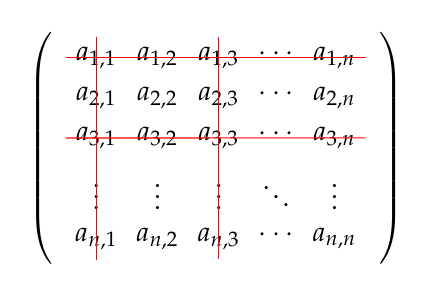
\begin{tikzpicture}
				\matrix (mat)[matrix of math nodes,left delimiter={(},right delimiter={)}]
				{%
					a_{1,1}  &  a_{1,2}  &  a_{1,3}  &  \cdots  &  a_{1,n} \\
					a_{2,1}  &  a_{2,2}  &  a_{2,3}  &  \cdots  &  a_{2,n} \\
					a_{3,1}  &  a_{3,2}  &  a_{3,3}  &  \cdots  &  a_{3,n} \\
					\vdots   &  \vdots   &  \vdots   &  \ddots  &  \vdots \\
					a_{n,1}  &  a_{n,2}  &  a_{n,3}  &  \cdots  &  a_{n,n} \\
				};
				
				\draw<2->[red] (mat-1-1.west) -- (mat-1-5.east);
				\draw<2->[red] (mat-3-1.west) -- (mat-3-5.east);
				\draw<2->[red] (mat-1-1.north) -- (mat-5-1.south);
				\draw<2->[red] (mat-1-3.north) -- (mat-5-3.south);
			\end{tikzpicture}
		\end{center}
		
		\textbf{Note:} The notation $ \Delta_k $ does not identify a unique  principal minor of order $ k $.
	\end{frame}
	
	\begin{frame}[fragile]
		\frametitle{Unconstrained Optimization in $ \mathbb{R}^n $}
		The $ k $-th \emph{leading principal minor} of a matrix $ A $ ($ 1\leq k \leq n $), denoted by $ D_k $, is the determinant of the submatrix \[  \begin{pmatrix}
			a_{1,1} & a_{1,2} & \cdots & a_{1,k}\\
			a_{2,1} & a_{2,2} & \cdots & a_{2,k}\\
			\vdots&\vdots& \ddots& \vdots\\
			a_{k,1} & a_{k,2} & \cdots & a_{k,k}
		\end{pmatrix} , \]
		i.e. the principal minor obtained by deleting the last $ n-k $ rows and columns and, respectively, keeping the first $ k $.
	\end{frame}
	
	\begin{frame}[fragile]
		\frametitle{Unconstrained Optimization in $ \mathbb{R}^n $}
		\begin{Fact}[Sylvester's criterion]
			Let $ A $ be a symmetric matrix. Then:
			\begin{enumerate}
				\item $ A $ is positive definite if and only if $ D_k >0,~k=1,\ldots,n $.
				\item $ A $ is positive semidefinite if and only if $ \Delta_k \geq 0 $ for all principal minors of order $ k = 1,\ldots,n $.
				\item $ A $ is negative definite if and only if $ (-1)^k D_k >0,~k=1,\ldots,n $.
				\item $ A $ is negative semidefinite if and only if $ (-1)^k \Delta_k \geq 0 $ for all principal minors of order $ k = 1,\ldots,n $.
			\end{enumerate}
			\label{fc:Sylvester}
		\end{Fact}
		
		Note that the necessary and sufficient conditions for ``semidefiniteness'' involve all principal minors (and hence are cumbersome to check), not just the leading principal minors.
	\end{frame}
	
	\begin{frame}[fragile]
		\frametitle{Unconstrained Optimization in $ \mathbb{R}^n $}
		Let a function $ f(\mathbf{x})=f(x_1,\ldots,x_n) $ be twice differentiable. The matrix of second partial derivatives, evaluated at a point $ \mathbf{x} $, i.e. \[ \begin{pmatrix}
			\dfrac{\partial^2 f(\mathbf{x})}{\partial x_1^2 } & \dfrac{\partial^2 f(\mathbf{x})}{\partial x_1 \partial x_2} & \cdots & \dfrac{\partial^2 f(\mathbf{x})}{\partial x_1 \partial x_n}\\[3ex]
			\dfrac{\partial^2 f(\mathbf{x})}{\partial x_2\partial x_1 } & \dfrac{\partial^2 f(\mathbf{x})}{\partial x_2^2} & \cdots & \dfrac{\partial^2 f(\mathbf{x})}{\partial x_2 \partial x_n}\\[3ex]
			\cdots & \cdots & \ddots & \cdots \\[3ex]
			\dfrac{\partial^2 f(\mathbf{x})}{\partial x_n \partial x_1 } & \dfrac{\partial^2 f(\mathbf{x})}{\partial x_n \partial x_2 } & \cdots & \dfrac{\partial^2 f(\mathbf{x})}{\partial x_n^2}
		\end{pmatrix} \] is called the \emph{Hessian (matrix)} of $ f $ at $ \mathbf{x} $.
	\end{frame}
	
	\begin{frame}[fragile]
		\frametitle{Unconstrained Optimization in $ \mathbb{R}^n $}
		\begin{itemize}
			\item The Hessian is denoted $ \mathbf{f''(x)} $. \bigskip
			\item The Hessian is symmetric. \bigskip
			\item Sometimes the partial derivative $ \dfrac{\partial^2 f(\mathbf{x})}{\partial x_i \partial x_j} $ is written as $ f''_{ij}(\mathbf{x}) $. \bigskip
			\item A leading principal minor of order $ k $ of the Hessian is denoted $ D_k(\mathbf{x}) $. \bigskip
			\item An arbitrary principal minor of order $ k $ of the Hessian is denoted $ \Delta_k(\mathbf{x}) $.
		\end{itemize}
		
	\end{frame}
	
	\begin{frame}[fragile]
		\frametitle{Unconstrained Optimization in $ \mathbb{R}^n $}
		\begin{Fact}
			Let a (twice) differentiable function $ f: \mathbb{R}^n \rightarrow \mathbb{R} $ have a critical point at $ \mathbf{x^*} $.
			\begin{enumerate}
				\item If the Hessian  $ \mathbf{f''(x^*)} $ is positive definite or, equivalently, $ D_k(\mathbf{x^*})>0,~k=1,\ldots,n $, then $ \mathbf{x^*} $ is a \emph{local minimum point}.
				\item If the Hessian  $ \mathbf{f''(x^*)} $ is negative definite or, equivalently, $ (-1)^k D_k(\mathbf{x^*})>0,~k=1,\ldots,n $, then $ \mathbf{x^*} $ is a \emph{local maximum point}.
				\item If $ D_n(\mathbf{x^*})\neq 0 $ and neither 1), nor 2) is satisfied, then $ \mathbf{x^*} $ is a \emph{saddle point}.
			\end{enumerate}
			\label{fc:ScsRn}
		\end{Fact}
	\end{frame}
	
	\begin{frame}[fragile]
		\frametitle{Unconstrained Optimization in $ \mathbb{R}^n $}
		\begin{Fact}
			Let a (twice) differentiable function $ f: \mathbb{R}^n \rightarrow \mathbb{R} $ have an extreme point at $ \mathbf{x^*} $.
			\begin{enumerate}
				\item If $ \mathbf{x^*} $ is a local minimum point, then the Hessian  $ \mathbf{f''(x^*)} $ is positive semidefinite or, equivalently, $ \Delta_k(\mathbf{x^*})\geq 0$ for all principal minors of order $ k=1,\ldots,n $.
				\item If $ \mathbf{x^*} $ is a local maximum point, then the Hessian  $ \mathbf{f''(x^*)} $ is negative semidefinite or, equivalently, $ (-1)^k \Delta_k(\mathbf{x^*})\geq 0$ for all principal minors of order $ k=1,\ldots,n $.
			\end{enumerate}
			\label{fc:NcsRn}
		\end{Fact}
	\end{frame}
	
	\begin{frame}[fragile]
		\frametitle{Unconstrained Optimization in $ \mathbb{R}^n $}
		\begin{exmpl}[Verification of Example \ref{ex:locminR2}] Recall that:
			\[ f(x,y) = x^2 +2y^2-3x+xy \]
			\[ \frac{\partial f}{\partial x} = 2x-3+y,\quad \frac{\partial f}{\partial y} = 4y+x.\]
			We now have:
			\[ \frac{\partial^2 f}{\partial x^2} = 2, \quad \frac{\partial^2 f}{\partial y^2} = 4,\quad \frac{\partial^2 f}{\partial x \partial y} = 1, \quad  \frac{\partial^2 f}{\partial y \partial x } = 1. \]
			
			\[ D_1 = \det (2) = 2>0, \quad D_2 = \det \begin{pmatrix}
				2 & 1\\
				1 & 4
			\end{pmatrix} = 2 \cdot 4 - 1 \cdot 1 = 7 > 0. \]
			
			Since $ D_1>0,~D_2>0 $, the critical point $ x=\frac{12}{7},~y=-\frac{3}{7} $ is a minimum.
			\label{ex:locminR2cont}
		\end{exmpl}
		
		%\textbf{Homework:} Apply the same procedure to Example \ref{ex:saddle}.
	\end{frame}
\end{section}


\begin{section}{Static Optimization with Equality Constraints. Lagrange Multipliers}\label{sec:Lagr}
	
	\begin{frame}[fragile]
		\frametitle{Static Optimization with Equality Constraints}
		\framesubtitle{Formulation}
		Now we look at problems of the form
		\begin{equation}
			f(x_1,\ldots,x_n)\rightarrow \min (\max)
			\label{eq:obj}
		\end{equation}
		s.t.
		\begin{equation}
			\begin{array}{l l l}
				g_1(x_1,\ldots,x_n) = b_1\\
				g_2(x_1,\ldots,x_n) = b_2\\
				\cdots \\
				g_m(x_1,\ldots,x_n) = b_m\\
			\end{array}
			\label{eq:constr}
		\end{equation}
		where $ m<n $. (Can you explain the last requirement?) \bigskip
		
		\textbf{Note:} In what follows, all required properties of the objects in \eqref{eq:obj} and \eqref{eq:constr} like differentiability are implicitly assumed.
	\end{frame}
	
	\begin{frame}[fragile]
		\frametitle{Static Optimization with Equality Constraints}
		\framesubtitle{Formulation}
		Using vector notation for compactness, the objective function is:
		\[ f(\mathbf{x}) \rightarrow \min (\max) \]
		We introduce
		\[ \mathbf{g}(\mathbf{x}):= (g_1(\mathbf{x}),\ldots,g_m(\mathbf{x}))',\quad \mathbf{b} = (b_1,\ldots,b_m)' \]
		and the constraints are written as 
		\[ \mathbf{g}(\mathbf{x})=\mathbf{b}. \]
	\end{frame}
	
	\begin{frame}[fragile]
		\frametitle{Static Optimization with Equality Constraints}
		\framesubtitle{The Lagrangian}
		The standard approach to solving \eqref{eq:obj}-\eqref{eq:constr} starts by defining a \emph{Lagrangian}:
		
		\[ \mathcal{L}(\mathbf{x}) = f(\mathbf{x}) - \lambda_1 (g_1(\mathbf{x})-b_1) - \cdots - \lambda_m (g_m(\mathbf{x})-b_m). \]\bigskip
		
		The numbers $ \lambda_1,\ldots,\lambda_m $ are called \emph{Lagrange multipliers}.\bigskip
		
		This can also be written in vector notation:
		\[ \mathcal{L}(\mathbf{x}) = f(\mathbf{x}) - \boldsymbol{\lambda}' (\mathbf{g}(\mathbf{x})-\mathbf{b}) , \] 
		where $ \boldsymbol{\lambda}= (\lambda_1,\ldots,\lambda_m)' $ is the vector of Lagrange multipliers. While, strictly speaking, $\mathcal{L}$ depends on $\boldsymbol{\lambda}$, we'll omit this dependence to lighten notation.  \bigskip
		
		\textbf{Note:} Here we follow the economics sign convention and subtract the constraint terms in the Lagrangian.
		Math textbooks typically use a ``+'' in front of $\lambda$; both lead to the same optimality conditions, with multipliers differing only by sign.
	\end{frame}
	
	\begin{frame}[fragile]
		\frametitle{Static Optimization with Equality Constraints}
		We can use the Lagrangian to produce candidates for optimality in the following manner:
		
		\begin{block}{Algorithm}
			\begin{enumerate}
				\item Form the Lagrangian as above
				\item Differentiate it w.r.t. the variables we are optimizing over, i.e.
				\[ \dfrac{\partial \mathcal{L}}{\partial x_i} = \dfrac{\partial f(\mathbf{x})}{\partial x_i} - \sum_{j=1}^{m}\lambda_j \dfrac{\partial g_j(\mathbf{x})}{\partial x_i},~i=1,\ldots,n \]
				\item Set the resulting derivatives equal to zero, i.e. construct the first-order conditions (FOCs)
				\begin{equation}
					 \dfrac{\partial \mathcal{L}}{\partial x_i} = 0,~i=1,\ldots,n
					\label{eq:Lagr_FOCs}
				\end{equation}
				\item The FOCs in the preceding step, together with the constraints \eqref{eq:constr}, form a system of $ n+m $ equations which is solved for the unknowns $ x_i $ and $ \lambda_j $
			\end{enumerate}
		\end{block}
	\end{frame}
	
	\begin{frame}[fragile]
		\frametitle{Static Optimization with Equality Constraints}
		\framesubtitle{Remarks}
		\begin{itemize}
			\item Sometimes the Lagrangian is formulated as \[ \mathcal{L}(\mathbf{x}) = f(\mathbf{x}) - \lambda_1 g_1(\mathbf{x}) - \cdots - \lambda_m g_m(\mathbf{x}). \] It obviously makes no difference in the differentiation step and produces the same result.
			\item One modification of the algorithm additionally requires differentiating the Lagrangian w.r.t. $ \lambda_j $ and setting the resulting derivatives equal to zero. This simply reproduces the constraints \eqref{eq:constr} and is covered by the last step of our algorithm.
			\item A Lagrange multiplier is interpreted as a \emph{shadow price}, i.e. the gain (or loss) arising from relaxing the associated constraint.
			\item The Lagrangian algorithm produces necessary conditions for optimality only under additional assumptions.
		\end{itemize}
	\end{frame}
	
	\begin{frame}[fragile]
		\frametitle{Static Optimization with Equality Constraints}
		\framesubtitle{Necessary conditions for optimality}
			
		\begin{Fact}
			Suppose that the functions $f$ and $g_1,\ldots,g_m$ are defined on a set
			$S$ in $\mathbb{R}^n$, and that $\mathbf{x}^* = (x_1^*,\ldots,x_n^*)$ is an
			interior point of $S$ that solves problem \eqref{eq:obj}-\eqref{eq:constr}. Suppose further that $f$ and
			$g_1,\ldots,g_m$ are $C^1$ in a ball around $\mathbf{x}^*$, and that the
			$m\times n$ matrix of partial derivatives of the constraint functions
			\[
			\mathbf{g}'(\mathbf{x}^*) =
			\begin{pmatrix}
				\dfrac{\partial g_1(\mathbf{x}^*)}{\partial x_1} & \cdots &
				\dfrac{\partial g_1(\mathbf{x}^*)}{\partial x_n} \\
				\vdots & \ddots & \vdots \\
				\dfrac{\partial g_m(\mathbf{x}^*)}{\partial x_1} & \cdots &
				\dfrac{\partial g_m(\mathbf{x}^*)}{\partial x_n}
			\end{pmatrix}
			\]
			has rank $m$. Then there exist unique numbers $\lambda_1,\ldots,\lambda_m$
			such that the solution $\mathbf{x}^*$ satisfies the FOCs \eqref{eq:Lagr_FOCs}.
			\label{fc:NC_Lagr}
		\end{Fact}
	\end{frame}
	
		\begin{frame}[fragile]
		\frametitle{Static Optimization with Equality Constraints}
		\framesubtitle{Sufficient conditions for optimality}
		
		\begin{Fact}
			If there exist numbers $\lambda_1,\ldots,\lambda_m$ and an admissible
			$\mathbf{x}^*$ which together satisfy the first-order conditions in the Lagrangian algorithm, and if
			the Lagrangian $\mathcal{L}(\mathbf{x})$ is concave (convex) in $\mathbf{x}$, and
			if $S$ is convex, then $\mathbf{x}^*$ solves the maximization (minimization)
			problem \eqref{eq:obj}-\eqref{eq:constr}.
			\label{fc:SC_Lagr}
		\end{Fact}
	\end{frame}
	
	\begin{frame}[fragile]
		\frametitle{Static Optimization with Equality Constraints}
		\framesubtitle{Local second-order conditions}
		\begin{itemize}\itemsep1em
			\item The sufficient conditions in Fact \ref{fc:SC_Lagr} are global and therefore often turn out to be too restrictive. A more widely applicable route to establishing optimality is given by \textit{local second-order conditions}.
			\item Local second-order conditions extend the unconstrained second-order test by replacing the Hessian of the objective function with an appropriate modification that incorporates the equality constraints.	
		\end{itemize}
	\end{frame}
		
		\begin{frame}[fragile]
			\frametitle{Static Optimization with Equality Constraints}
			\framesubtitle{Local second-order conditions: bordered Hessians}
			 For problem \eqref{eq:obj}-\eqref{eq:constr} and $r=m+1,\ldots,n$ we define the \textbf{bordered Hessian determinant} as follows:
			\[
			B_r(\mathbf{x}^*) =
			\begin{vmatrix}
				0 & \cdots & 0
				& \dfrac{\partial g_1(\mathbf{x}^*)}{\partial x_1}
				& \cdots
				& \dfrac{\partial g_1(\mathbf{x}^*)}{\partial x_r} \\[1ex]
				\vdots & \ddots & \vdots
				& \vdots & & \vdots \\[1ex]
				0 & \cdots & 0
				& \dfrac{\partial g_m(\mathbf{x}^*)}{\partial x_1}
				& \cdots
				& \dfrac{\partial g_m(\mathbf{x}^*)}{\partial x_r} \\[1ex]
				\dfrac{\partial g_1(\mathbf{x}^*)}{\partial x_1}
				& \cdots
				& \dfrac{\partial g_m(\mathbf{x}^*)}{\partial x_1}
				& \dfrac{\partial^2 \mathcal L(\mathbf{x}^*)}{\partial x_1^2}
				& \cdots
				& \dfrac{\partial^2 \mathcal L(\mathbf{x}^*)}{\partial x_1 \partial x_r} \\[1ex]
				\vdots & & \vdots
				& \vdots & \ddots & \vdots \\[1ex]
				\dfrac{\partial g_1(\mathbf{x}^*)}{\partial x_r}
				& \cdots
				& \dfrac{\partial g_m(\mathbf{x}^*)}{\partial x_r}
				& \dfrac{\partial^2 \mathcal L(\mathbf{x}^*)}{\partial x_r \partial x_1}
				& \cdots
				& \dfrac{\partial^2 \mathcal L(\mathbf{x}^*}{\partial x_r^2}
			\end{vmatrix}
			\]
		\end{frame}
	
	\begin{frame}[fragile]
		\frametitle{Static Optimization with Equality Constraints}
		\framesubtitle{Remarks on bordered Hessians}
		\begin{itemize}\itemsep1em
			\item Some expositions directly define the full bordered Hessian matrix (the matrix under the determinant sign in the previous slide in the case $r=n$) and then discuss the last $n-m$ leading principal minors of this matrix, which of course are our objects $B_r(\mathbf{x}^*)$, $r=m+1,\ldots,n$.
			\item One way of compactly describing the matrix underlying a bordered Hessian determinant is to say it has the following block structure:
			\[ \begin{pmatrix}
				\mathbf{0}_{m \times m} & J_{m \times r} \\[1ex]
				J'_{r \times m} & H_{r \times r}
			\end{pmatrix}, \]
			where $J$ denotes the (partial) Jacobian of the vector function specifying the constraints, $H$ is the (partial) Hessian of the Lagrangian function and the subscripts indicate the dimensions of the corresponding matrices.
			\item We may need to re-label variables to ensure that the first $m$ columns of the $J_{m \times r}$ matrix are linearly independent. This is assumed in what follows.
		\end{itemize}
	\end{frame}
	
	
	\begin{frame}[fragile]
		\frametitle{Static Optimization with Equality Constraints}
		\framesubtitle{Local second-order conditions: the general case}
		The following second-derivative test provides ``local'' sufficient conditions for optimality:
		\begin{Fact}
			Suppose the functions $f$ and $g_1,\ldots,g_m$ are defined on a set $S\subset\mathbb{R}^n$, and let
			$\mathbf{x}^*$ be an interior point of $S$ satisfying the necessary conditions in Fact \ref{fc:NC_Lagr}.
			Suppose further that $f$ and $g_1,\ldots,g_m$ are $C^2$ in a ball around $\mathbf{x}^*$.
			With the determinants $B_r(\mathbf{x}^*)$ defined as above, we have:
			\begin{enumerate}
				\item If $(-1)^m\,B_r(\mathbf{x}^*)>0$ for $r=m+1,\ldots,n$, then $\mathbf{x}^*$ solves the local
				minimization problem in \eqref{eq:obj}-\eqref{eq:constr}.
				\item If $(-1)^r\,B_r(\mathbf{x}^*)>0$ for $r=m+1,\ldots,n$, then $\mathbf{x}^*$ solves the local
				maximization problem in \eqref{eq:obj}-\eqref{eq:constr}.
			\end{enumerate}
		\end{Fact}\bigskip
		
		Note that the first condition requires the bordered Hessian determinants to keep the same sign, while the second one requires that the signs alternate.
	\end{frame}
	
	\begin{frame}[fragile]
		\frametitle{Static Optimization with Equality Constraints}
		\framesubtitle{Local second-order conditions: one constraint (setup)}
		
		Consider the common case of a \textbf{single} equality constraint ($m=1$):
		\[
		f(\mathbf{x}) \to \max~(\min)
		\quad \text{s.t.} \quad g(\mathbf{x})=b,
		\qquad \mathbf{x}\in S\subset\mathbb{R}^n.
		\]
		
		For $r=2,\ldots,n$, the \textbf{bordered Hessian determinant} (restricted to $x_1,\ldots,x_r$) takes the form
		\[
		B_r(\mathbf{x}^*)=
		\begin{vmatrix}
			0 & \nabla g_r(\mathbf{x}^*)' \\[0.5ex]
			\nabla g_r(\mathbf{x}^*) & H_r(\mathbf{x}^*)
		\end{vmatrix},
		\]
		where
		\[
		\nabla g_r(\mathbf{x}^*) =
		\begin{pmatrix}
			\dfrac{\partial g(\mathbf{x}^*)}{\partial x_1}\\ \vdots\\ \dfrac{\partial g(\mathbf{x}^*)}{\partial x_r}
		\end{pmatrix},
		\qquad
		H_r(\mathbf{x}^*)=
		\left[\dfrac{\partial^2 \mathcal{L}(\mathbf{x}^*)}{\partial x_i\,\partial x_j}\right]_{i,j=1,\ldots,r}.
		\]
		
		
	\end{frame}
	
	
	\begin{frame}[fragile]
		\frametitle{Static Optimization with Equality Constraints}
		\framesubtitle{Local second-order conditions: one constraint (test)}
		
		Suppose $\mathbf{x}^*$ is an admissible point satisfying the first-order conditions
		for the Lagrangian method with one equality constraint, and assume the required $C^2$
		regularity in a neighborhood of $\mathbf{x}^*$.
		
		\begin{block}{Second-derivative test ($m=1$)}
			For the determinants $B_r(\mathbf{x}^*)$ from the previous slide:
			\begin{itemize}\itemsep0.6em
				\item \textbf{Local maximum:} $(-1)^r\,B_r(\mathbf{x}^*)>0$ for $r=2,\ldots,n$.
				\item \textbf{Local minimum:} $-B_r(\mathbf{x}^*)>0$ for $r=2,\ldots,n$
				(equivalently, $B_r(\mathbf{x}^*)<0$ for all $r$).
			\end{itemize}
		\end{block}
		
		\smallskip
		\textbf{Remark:} The local maximum condition requires alternating signs across $r$,
		while the local minimum condition requires the same sign across $r$.
	\end{frame}
	
	
	
	
	
	
	
	
	
	\begin{frame}[fragile]
		\frametitle{Static Optimization with Equality Constraints}
		\begin{exmpl}[Basic intertemporal optimization]
			\begin{itemize}
				\item An economic agent lives for two periods and supplies a fixed amount of labour in the first period of his life in exchange for monetary payment $ y $.
				\item In period $ 1 $ the agent consumes $ c_1 $ units of a good out of his income and saves the remaining $ y-c_1 $.  (For convenience we assume there is no inflation and the price of the good is normalized to one.)
				\item Savings are remunerated at an interest rate $ r $. Thus, in the second period the agent has at his disposal \[ (y-c_1)(1+r) \] to finance consumption, denoted $ c_2 $.
				\item  The agent obtains utility from consumption according to the utility function
				\[ u(c_1,c_2) = \ln c_1 + \beta \ln c_2,~\beta \in (0,1) . \]
				\item The agent seeks to maximize utility w.r.t. $ c_1,c_2 $.
			\end{itemize}
			\label{ex:intertemp}
		\end{exmpl}
	\end{frame}
	
	\begin{frame}[fragile]
		\frametitle{Static Optimization with Equality Constraints}
		\addtocounter{exmpl}{-1}
		\begin{exmpl}[cont.]
			The above problem can be formalized as \[  \max_{c_1,c_2} u(c_1,c_2) \]
			s.t. \[ c_2 = (y-c_1)(1+r). \]
			
			Notice that the constraint can be written equivalently as \[ c_1 + \dfrac{c_2}{1+r} = y \] to conform to the $ \mathbf{g}(\mathbf{x})=\mathbf{b} $ convention. (Can you interpret the last equation in terms of discounting to period 1 quantities?)
			
			The Lagrangian for this problem is \[ \mathcal{L} = \ln c_1 + \beta \ln c_2 - \lambda \left(  c_1 + \frac{c_2}{1+r} - y \right). \]
		\end{exmpl}
	\end{frame}
	
	\begin{frame}[fragile]
		\frametitle{Static Optimization with Equality Constraints}
		\addtocounter{exmpl}{-1}
		\begin{exmpl}[cont.] The solution algorithm yields
			\[ \dfrac{\partial \mathcal{L}}{\partial c_1} = \dfrac{1}{c_1} - \lambda = 0 \quad \Rightarrow \quad c_1 = \dfrac{1}{\lambda} \]
			\[ \dfrac{\partial \mathcal{L}}{\partial c_2} = \beta \dfrac{1}{c_2} - \dfrac{\lambda}{1+r} = 0 \quad \Rightarrow \quad c_2 = \dfrac{\beta (1+r)}{\lambda} \]
			
			Combining the above equations to eliminate $ \lambda $, we obtain \[ c_2 = \beta (1+r)c_1. \]
			
			Substitute the last expression in the budget constraint:
			\[ c_1 + \dfrac{\beta (1+r)c_1}{1+r} = y \quad \Rightarrow \quad c_1^* = \dfrac{y}{1+\beta}.\]
		\end{exmpl}
	\end{frame}
	
	\begin{frame}[fragile]
		\frametitle{Static Optimization with Equality Constraints}
		\addtocounter{exmpl}{-1}
		\begin{exmpl}[cont.] 
			We then have \[ c_2^* = \beta (1+r)c_1 =  (1+r)\dfrac{\beta}{1+\beta}y. \]
						
			\textbf{Second-order condition (bordered Hessian)}
			
			The constraint is $g(c_1,c_2)=c_1+\dfrac{c_2}{1+r}=y$, hence
			\[
			\frac{\partial g}{\partial c_1}=1,
			\qquad
			\frac{\partial g}{\partial c_2}=\frac{1}{1+r}.
			\]
			The Hessian of the Lagrangian w.r.t.\ $(c_1,c_2)$ is
			\[
			H=
			\begin{pmatrix}
				\dfrac{\partial^2\mathcal L}{\partial c_1^2} & \dfrac{\partial^2\mathcal L}{\partial c_1\partial c_2}\\[1ex]
				\dfrac{\partial^2\mathcal L}{\partial c_2\partial c_1} & \dfrac{\partial^2\mathcal L}{\partial c_2^2}
			\end{pmatrix}
			=
			\begin{pmatrix}
				-\dfrac{1}{c_1^2} & 0\\[1ex]
				0 & -\dfrac{\beta}{c_2^2}
			\end{pmatrix}.
			\]
		\end{exmpl}
	\end{frame}
	
	
	\begin{frame}[fragile]
		\frametitle{Static Optimization with Equality Constraints}
		\addtocounter{exmpl}{-1}
		\begin{exmpl}[cont.] 
			Since $n=2$ and $m=1$, we only need $B_2$:
			\[
			B_2(\mathbf{x}^*)=
			\begin{vmatrix}
				0 & 1 & \dfrac{1}{1+r}\\[1ex]
				1 & -\dfrac{1}{(c_1^*)^2} & 0\\[1ex]
				\dfrac{1}{1+r} & 0 & -\dfrac{\beta}{(c_2^*)^2}
			\end{vmatrix}
			=
			\frac{\beta}{(c_2^*)^2}+\frac{1}{(1+r)^2}\frac{1}{(c_1^*)^2}
			\;>\;0.
			\]
			
			Therefore $(-1)^2B_2(\mathbf{x}^*)>0$, so $(c_1^*,c_2^*)$ is a \textbf{local maximum}.
		\end{exmpl}
	\end{frame}
	
	
	
	\begin{frame}[fragile]
		\frametitle{Static Optimization with Equality Constraints}
		\addtocounter{exmpl}{-1}
		\begin{exmpl}[cont.] 
			
			Let us check how the optimal value of the utility function $u^*= u(c_1^*,c_2^*) $ changes with income: 
			\[ \begin{split}
				\dfrac{\partial u^*}{\partial y} = & \dfrac{\partial }{\partial y} \left( \ln \dfrac{y}{1+\beta} + \beta \ln  \dfrac{(1+r)\beta y}{1+\beta} \right)\\ {}\\
				= & \dfrac{1+\beta}{y}\dfrac{1}{1+\beta} + \beta \dfrac{1+\beta}{(1+r)\beta y} \dfrac{(1+r)\beta }{1+\beta} \\{}\\
				= & \dfrac{1}{y}+\dfrac{\beta}{y} = \dfrac{1+\beta}{y}  \uncover<2->{\color{red}{= \dfrac{1}{c_1^*} = \lambda. \quad \text{Interpretation?}}}
			\end{split}\] 
		\end{exmpl}
	\end{frame}
	
	%\begin{frame}[fragile]
	%\frametitle{Static Optimization with Equality Constraints}
	%\textbf{Homework:} Check that the Lagrangian in Example \ref{ex:intertemp} is concave in $ c_1,c_2 $ to convince yourself that the algorithm indeed produces a maximum. \bigskip
	%
	%\textbf{Homework:} What are the conditions on the model parameters (i.e. on $ y,r,\beta $) in Example \ref{ex:intertemp} that ensure that consumption will be equal between the two periods? What are the conditions to have $ c_1 > c_2 $? What's the economic intuition for that?
	%\end{frame}
	
\end{section}

\begin{frame}[fragile]
	\frametitle{Readings}
	\textbf{Main references:}
	
	Syds\ae{}ter et al. [SHSS] \emph{Further mathematics for economic analysis}. Chapter 3.\bigskip
	
	\textbf{Additional readings:}
	
	Simon and Blume. \emph{Mathematics for economists}. Chapters 17 and 18.
\end{frame}

\end{document}